% Options for packages loaded elsewhere
\PassOptionsToPackage{unicode}{hyperref}
\PassOptionsToPackage{hyphens}{url}
%
\documentclass[
  12pt,
  a4paper,
  DIV=11,
  numbers=noendperiod]{scrreprt}

\usepackage{amsmath,amssymb}
\usepackage{setspace}
\usepackage{iftex}
\ifPDFTeX
  \usepackage[T1]{fontenc}
  \usepackage[utf8]{inputenc}
  \usepackage{textcomp} % provide euro and other symbols
\else % if luatex or xetex
  \usepackage{unicode-math}
  \defaultfontfeatures{Scale=MatchLowercase}
  \defaultfontfeatures[\rmfamily]{Ligatures=TeX,Scale=1}
\fi
\usepackage{lmodern}
\ifPDFTeX\else  
    % xetex/luatex font selection
\fi
% Use upquote if available, for straight quotes in verbatim environments
\IfFileExists{upquote.sty}{\usepackage{upquote}}{}
\IfFileExists{microtype.sty}{% use microtype if available
  \usepackage[]{microtype}
  \UseMicrotypeSet[protrusion]{basicmath} % disable protrusion for tt fonts
}{}
\usepackage{xcolor}
\setlength{\emergencystretch}{3em} % prevent overfull lines
\setcounter{secnumdepth}{5}
% Make \paragraph and \subparagraph free-standing
\ifx\paragraph\undefined\else
  \let\oldparagraph\paragraph
  \renewcommand{\paragraph}[1]{\oldparagraph{#1}\mbox{}}
\fi
\ifx\subparagraph\undefined\else
  \let\oldsubparagraph\subparagraph
  \renewcommand{\subparagraph}[1]{\oldsubparagraph{#1}\mbox{}}
\fi


\providecommand{\tightlist}{%
  \setlength{\itemsep}{0pt}\setlength{\parskip}{0pt}}\usepackage{longtable,booktabs,array}
\usepackage{calc} % for calculating minipage widths
% Correct order of tables after \paragraph or \subparagraph
\usepackage{etoolbox}
\makeatletter
\patchcmd\longtable{\par}{\if@noskipsec\mbox{}\fi\par}{}{}
\makeatother
% Allow footnotes in longtable head/foot
\IfFileExists{footnotehyper.sty}{\usepackage{footnotehyper}}{\usepackage{footnote}}
\makesavenoteenv{longtable}
\usepackage{graphicx}
\makeatletter
\def\maxwidth{\ifdim\Gin@nat@width>\linewidth\linewidth\else\Gin@nat@width\fi}
\def\maxheight{\ifdim\Gin@nat@height>\textheight\textheight\else\Gin@nat@height\fi}
\makeatother
% Scale images if necessary, so that they will not overflow the page
% margins by default, and it is still possible to overwrite the defaults
% using explicit options in \includegraphics[width, height, ...]{}
\setkeys{Gin}{width=\maxwidth,height=\maxheight,keepaspectratio}
% Set default figure placement to htbp
\makeatletter
\def\fps@figure{htbp}
\makeatother

\KOMAoption{captions}{tableheading}
\usepackage{indentfirst}
\usepackage{float}
\floatplacement{figure}{H}
\usepackage[math,RM={Scale=0.94},SS={Scale=0.94},SScon={Scale=0.94},TT={Scale=MatchLowercase,FakeStretch=0.9},DefaultFeatures={Ligatures=Common}]{plex-otf}
\makeatletter
\@ifpackageloaded{caption}{}{\usepackage{caption}}
\AtBeginDocument{%
\ifdefined\contentsname
  \renewcommand*\contentsname{Содержание}
\else
  \newcommand\contentsname{Содержание}
\fi
\ifdefined\listfigurename
  \renewcommand*\listfigurename{Список иллюстраций}
\else
  \newcommand\listfigurename{Список иллюстраций}
\fi
\ifdefined\listtablename
  \renewcommand*\listtablename{Список таблиц}
\else
  \newcommand\listtablename{Список таблиц}
\fi
\ifdefined\figurename
  \renewcommand*\figurename{Рисунок}
\else
  \newcommand\figurename{Рисунок}
\fi
\ifdefined\tablename
  \renewcommand*\tablename{Таблица}
\else
  \newcommand\tablename{Таблица}
\fi
}
\@ifpackageloaded{float}{}{\usepackage{float}}
\floatstyle{ruled}
\@ifundefined{c@chapter}{\newfloat{codelisting}{h}{lop}}{\newfloat{codelisting}{h}{lop}[chapter]}
\floatname{codelisting}{Список}
\newcommand*\listoflistings{\listof{codelisting}{Листинги}}
\makeatother
\makeatletter
\makeatother
\makeatletter
\@ifpackageloaded{caption}{}{\usepackage{caption}}
\@ifpackageloaded{subcaption}{}{\usepackage{subcaption}}
\makeatother
\ifLuaTeX
\usepackage[bidi=basic]{babel}
\else
\usepackage[bidi=default]{babel}
\fi
\babelprovide[main,import]{russian}
\babelprovide[import]{english}
% get rid of language-specific shorthands (see #6817):
\let\LanguageShortHands\languageshorthands
\def\languageshorthands#1{}
\ifLuaTeX
  \usepackage{selnolig}  % disable illegal ligatures
\fi
\usepackage[style=gost-numeric,backend=biber,langhook=extras,autolang=other*]{biblatex}
\addbibresource{bib/cite.bib}
\usepackage{csquotes}
\usepackage{bookmark}

\IfFileExists{xurl.sty}{\usepackage{xurl}}{} % add URL line breaks if available
\urlstyle{same} % disable monospaced font for URLs
\hypersetup{
  pdftitle={Отчет по лабораторной работе 5},
  pdfauthor={Власов Артем Сергеевич},
  pdflang={ru-RU},
  hidelinks,
  pdfcreator={LaTeX via pandoc}}

\title{Отчет по лабораторной работе 5}
\usepackage{etoolbox}
\makeatletter
\providecommand{\subtitle}[1]{% add subtitle to \maketitle
  \apptocmd{\@title}{\par {\large #1 \par}}{}{}
}
\makeatother
\subtitle{Власов Артем Сергеевич}
\author{Власов Артем Сергеевич}
\date{}

\begin{document}
\maketitle

\renewcommand*\contentsname{Содержание}
{
\setcounter{tocdepth}{1}
\tableofcontents
}
\listoffigures
\listoftables
\setstretch{1.5}
\chapter{Цель
работы}\label{ux446ux435ux43bux44c-ux440ux430ux431ux43eux442ux44b}

Получить навыки управления системными службами операционной системы
посредством systemd.

\chapter{Задание}\label{ux437ux430ux434ux430ux43dux438ux435}

Выполнить действия по запуску, определению статуса добавлению в
автозапуск службы Very Secure FTP. Получить навыки для разрешения
конфликта служб iptables и firewalld. Продемонстрировать навыки работы с
изолированными целями.

\chapter{Выполнение лабораторной работы
5.}\label{ux432ux44bux43fux43eux43bux43dux435ux43dux438ux435-ux43bux430ux431ux43eux440ux430ux442ux43eux440ux43dux43eux439-ux440ux430ux431ux43eux442ux44b-5.}

Переходим на пользователя root и устанавливаем vsftpd.

\begin{figure}

{\centering 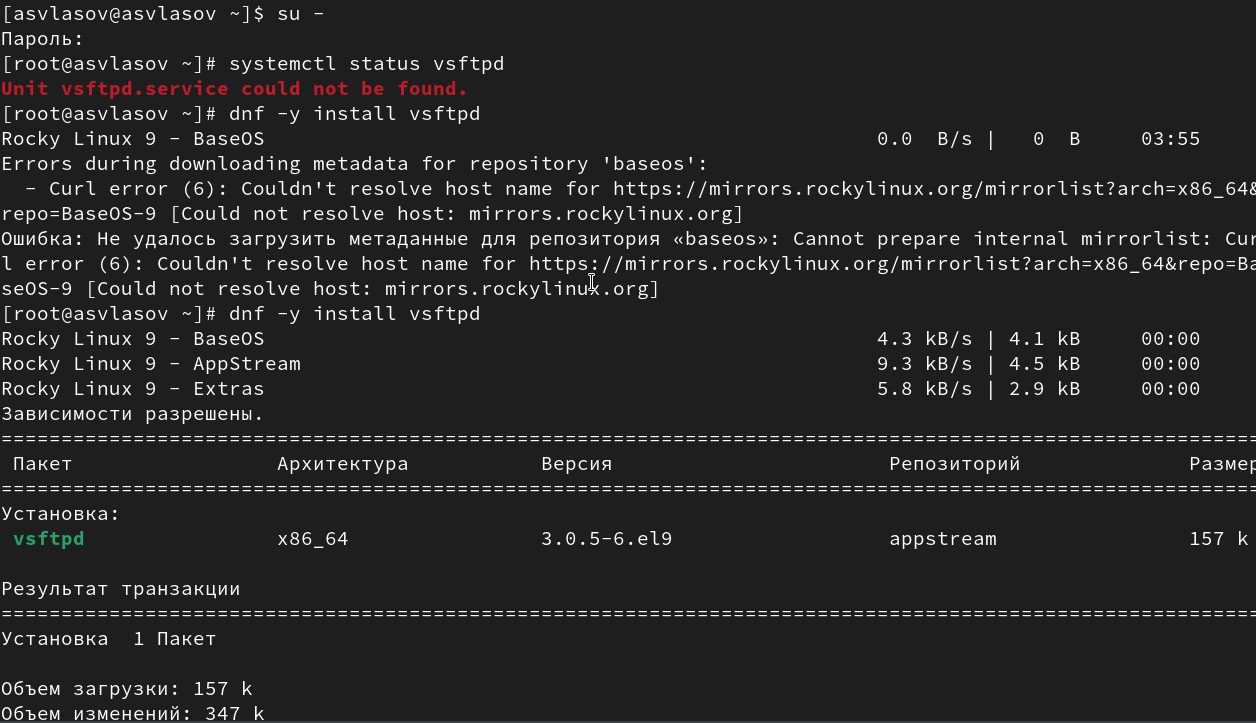
\includegraphics[width=0.7\textwidth,height=\textheight]{image/1.png}

}

\caption{vsftpd}

\end{figure}%

Смотрим статус службы, затем добавив службу в автозапуск смотрим статус
еще раз.

\begin{figure}

{\centering 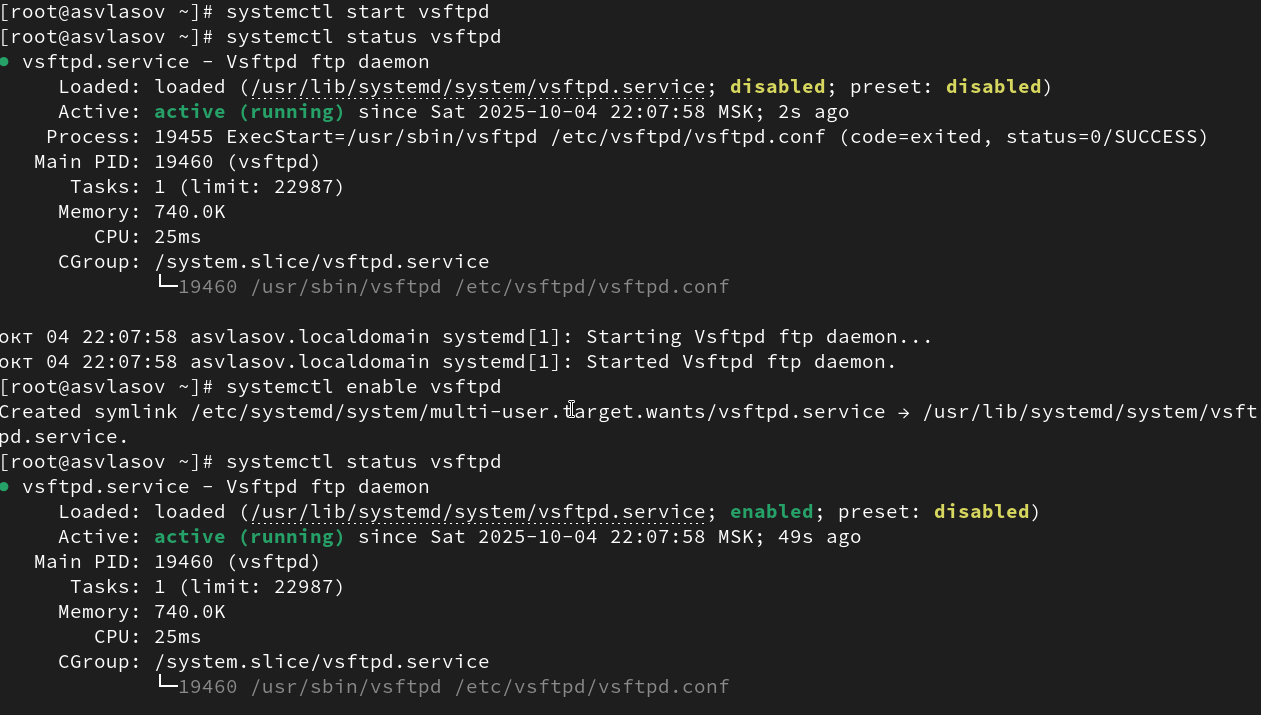
\includegraphics[width=0.7\textwidth,height=\textheight]{image/2.png}

}

\caption{Статус службы}

\end{figure}%

Убираем службу из автозапуска и смотрим снова.

\begin{figure}

{\centering 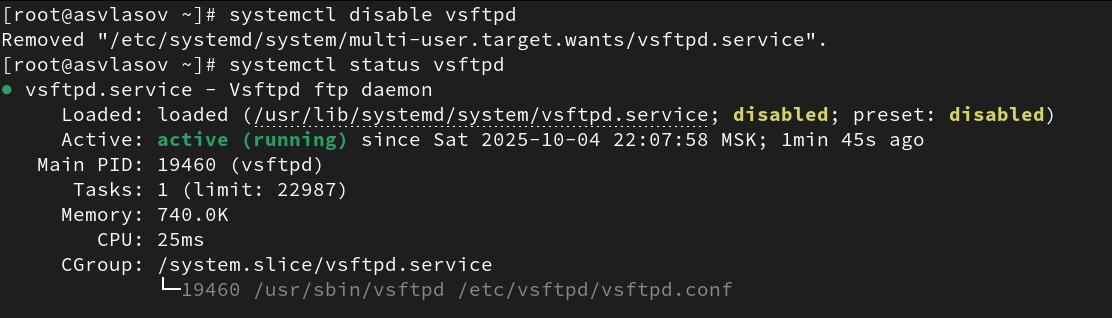
\includegraphics[width=0.7\textwidth,height=\textheight]{image/3.png}

}

\caption{Статус изменения}

\end{figure}%

Выводим на экран символические ссылки запуска служб.

\begin{figure}

{\centering 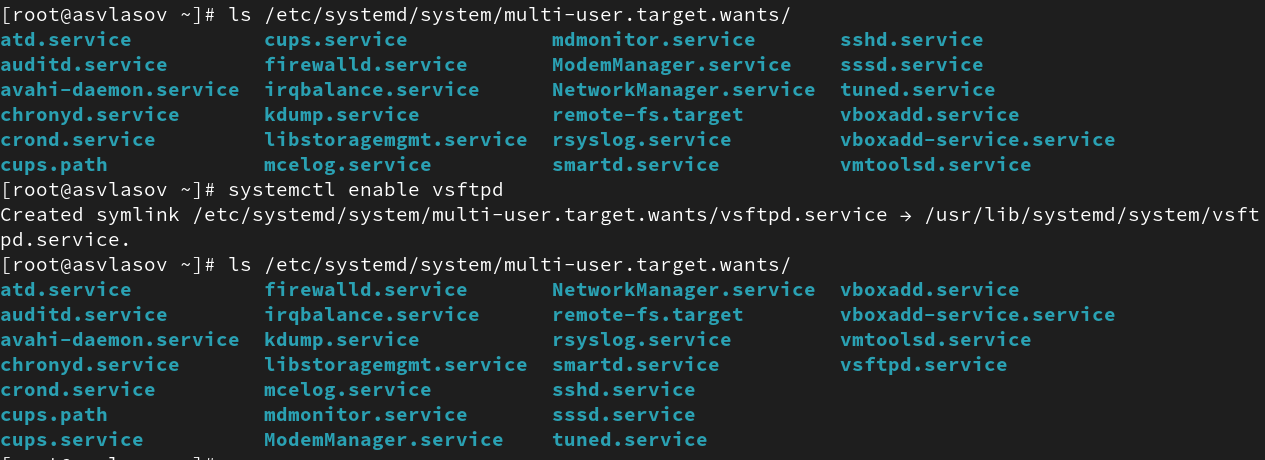
\includegraphics[width=0.7\textwidth,height=\textheight]{image/4.png}

}

\caption{Символические ссылки}

\end{figure}%

Видим, что если включить службу в автозапуск, она появляется в
символических ссылках.

Выводим на экран список зависимостей юнита

\begin{figure}

{\centering 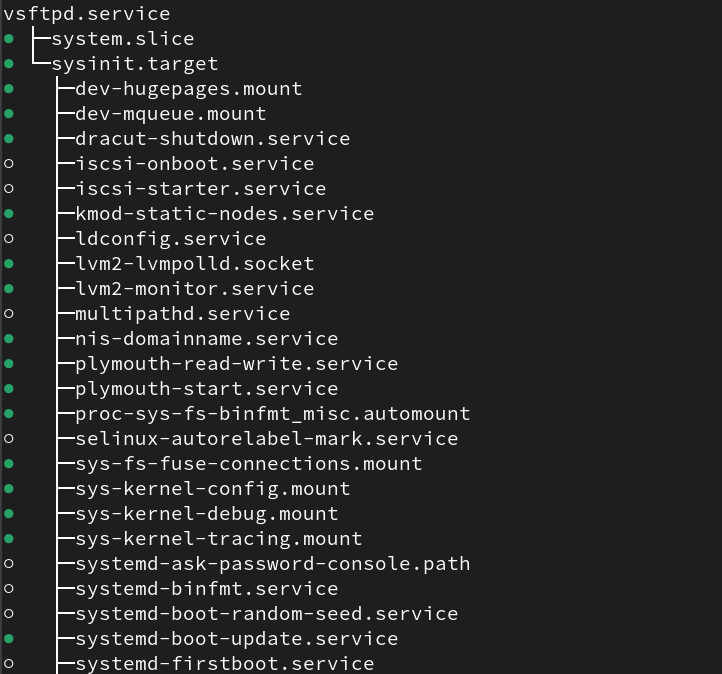
\includegraphics[width=0.7\textwidth,height=\textheight]{image/5.png}

}

\caption{Юниты}

\end{figure}%

Далее выводим список юнитов, зависимых от нашего.

\begin{figure}

{\centering 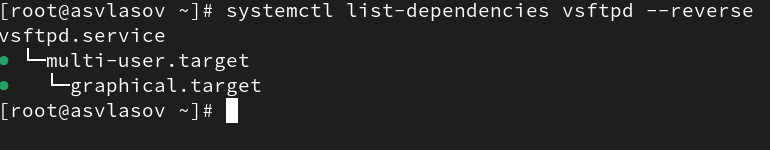
\includegraphics[width=0.7\textwidth,height=\textheight]{image/6.png}

}

\caption{Зависимые юниты}

\end{figure}%

Проверяем статус служб iptables и firewalld после установки. Затем
запускаем службы, видим конфликт.

\begin{figure}

{\centering 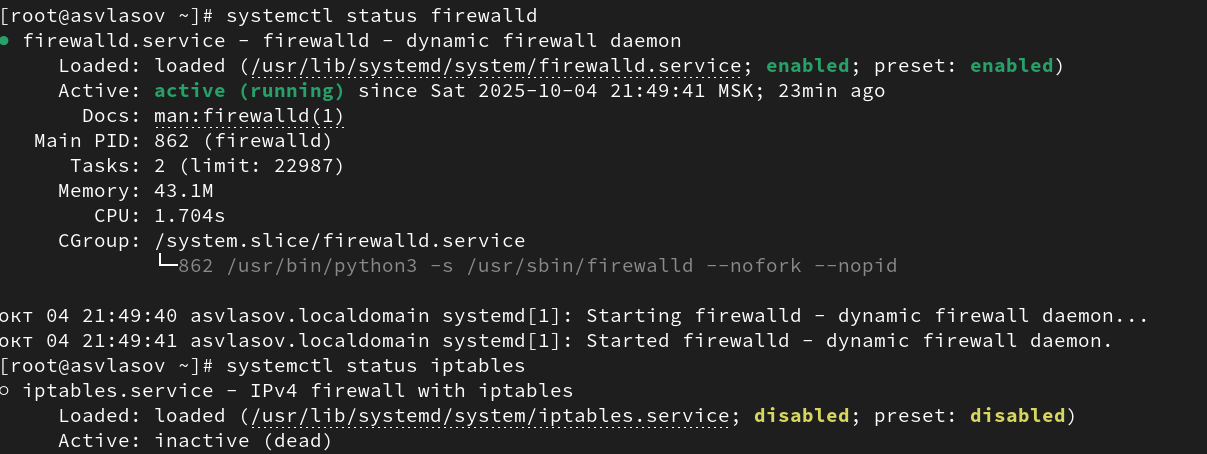
\includegraphics[width=0.7\textwidth,height=\textheight]{image/7.png}

}

\caption{Статус служб}

\end{figure}%

Провеярем настройки служб

\begin{figure}

{\centering 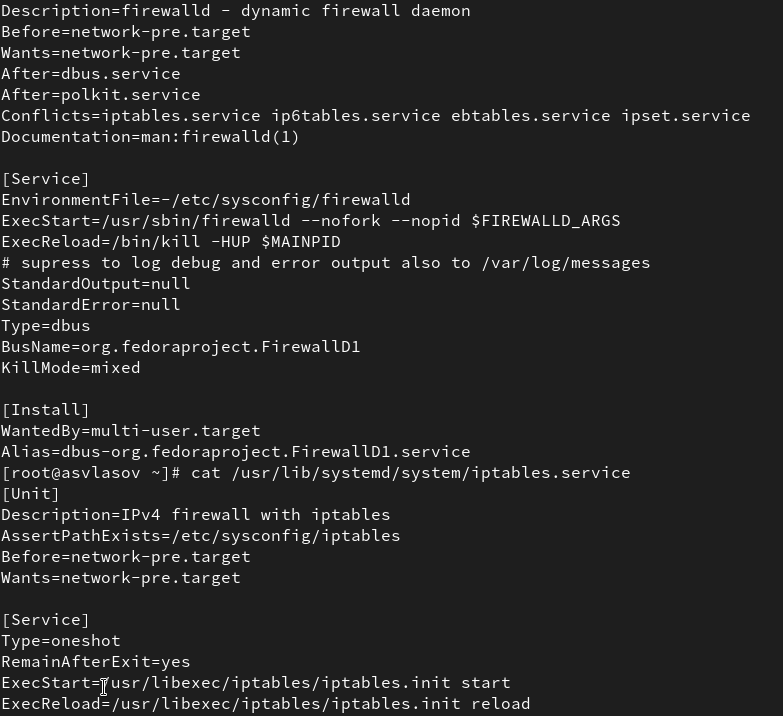
\includegraphics[width=0.7\textwidth,height=\textheight]{image/8.png}

}

\caption{Настройки служб}

\end{figure}%

Выгружаем службу iptables. Затем запускаем вторую службу, все приходит в
норму. Блокируем запуск службы iptables и проверяем. Пробуем запустить
iptables. Ошибка.

\begin{figure}

{\centering 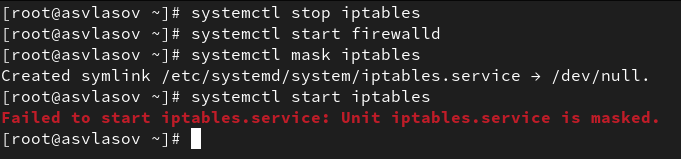
\includegraphics[width=0.7\textwidth,height=\textheight]{image/9.png}

}

\caption{Блокировка службы}

\end{figure}%

Пробуем поставить службу в автозапуск.

\begin{figure}

{\centering 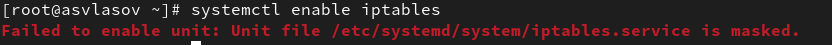
\includegraphics[width=0.7\textwidth,height=\textheight]{image/10.png}

}

\caption{Ошибка}

\end{figure}%

Список всех целей для изолирования. И загрузка системы в режиме
восстановления.

\begin{figure}

{\centering 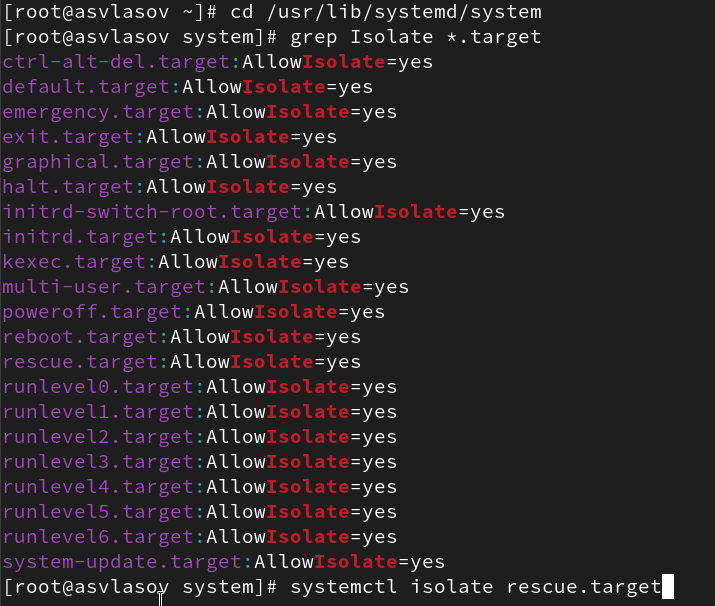
\includegraphics[width=0.7\textwidth,height=\textheight]{image/12.png}

}

\caption{Изолирование}

\end{figure}%

Проверка режима восстановления.

\begin{figure}

{\centering 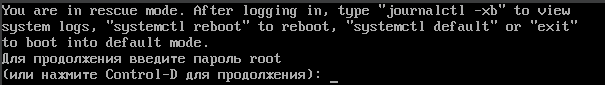
\includegraphics[width=0.7\textwidth,height=\textheight]{image/11.png}

}

\caption{Режим восстановления}

\end{figure}%

Перезагрузка системы с помощью isolate.

\begin{figure}

{\centering 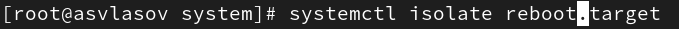
\includegraphics[width=0.7\textwidth,height=\textheight]{image/13.png}

}

\caption{Перезагрузка}

\end{figure}%

Запускаем систему с текстовом режиме с помощью multi-user.target. В
текстовом режиме возвращаем графический режим.

\begin{figure}

{\centering 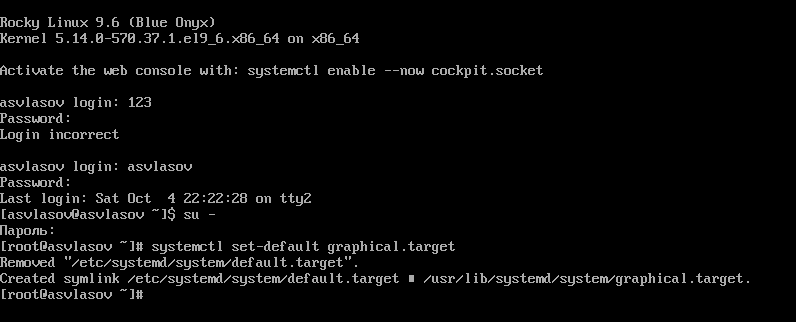
\includegraphics[width=0.7\textwidth,height=\textheight]{image/14.png}

}

\caption{Текстовый режим}

\end{figure}%

Проверка графического режима.

\begin{figure}

{\centering 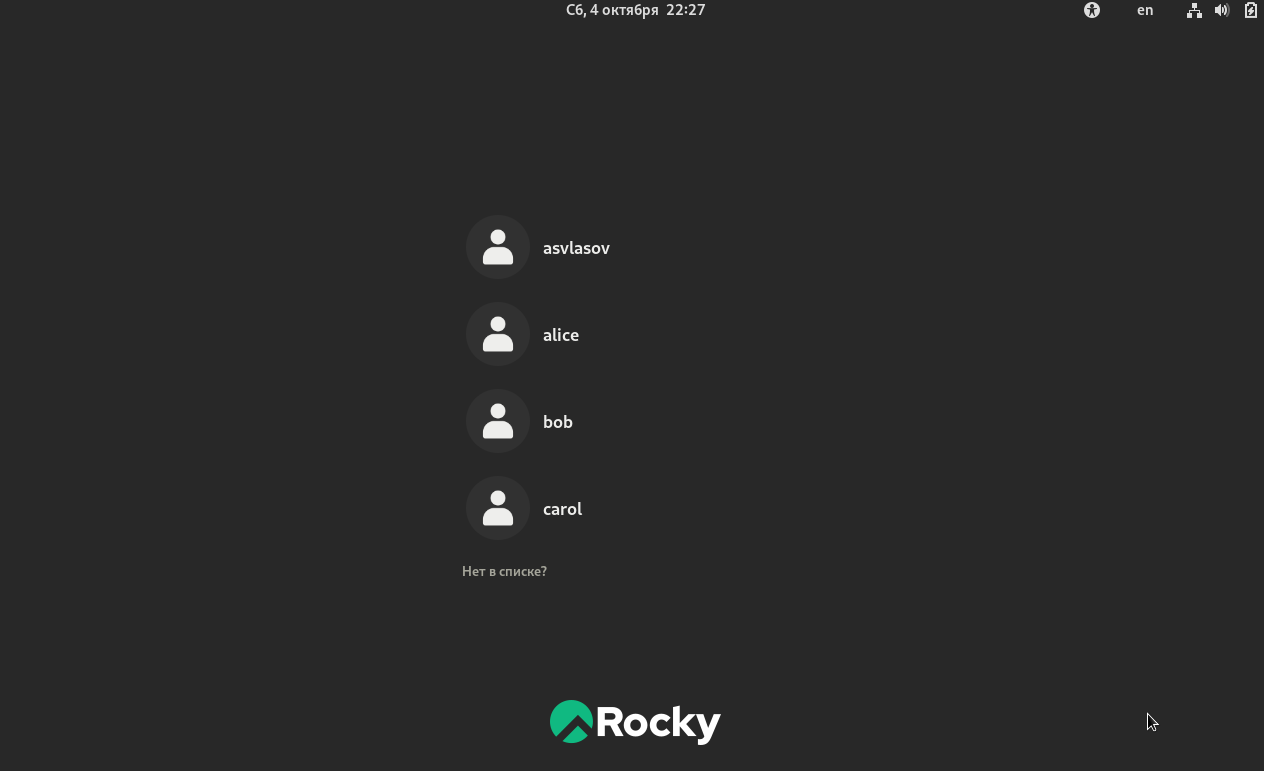
\includegraphics[width=0.7\textwidth,height=\textheight]{image/15.png}

}

\caption{Графический режим}

\end{figure}%

\#Контрольные вопросы

\begin{enumerate}
\def\labelenumi{\arabic{enumi}.}
\item
  Какая команда позволяет вам искать пакет rpm, содержащий файл useradd?
  dnf provides */useradd или rpm -qf /usr/sbin/useradd (если файл уже
  установлен)
\item
  Какие команды вам нужно использовать, чтобы показать имя группы dnf,
  которая содержит инструменты безопасности и показывает, что находится
  в этой группе? dnf group list (для просмотра групп) и dnf group info
  \enquote{Имя\_группы\_безопасности}
\item
  Какая команда позволяет вам установить rpm, который вы загрузили из
  Интернета и который не находится в репозиториях? dnf install
  /путь/к/файлу.rpm или rpm -i /путь/к/файлу.rpm
\item
  Вы хотите убедиться, что пакет rpm, который вы загрузили, не содержит
  никакого опасного кода сценария. Какая команда позволяет это сделать?
  rpm --checksig /путь/к/файлу.rpm или rpm -K /путь/к/файлу.rpm
\item
  Какая команда показывает всю документацию в rpm? rpm -qd имя\_пакета
\item
  Какая команда показывает, какому пакету rpm принадлежит файл? rpm -qf
  /путь/к/файлу
\end{enumerate}

\chapter{Выводы}\label{ux432ux44bux432ux43eux434ux44b}

Мы получили навыки управления системными службами операционной системы
посредством systemd.

\chapter*{Список
литературы}\label{ux441ux43fux438ux441ux43eux43a-ux43bux438ux442ux435ux440ux430ux442ux443ux440ux44b}
\addcontentsline{toc}{chapter}{Список литературы}

\printbibliography[heading=none]




\end{document}
